\section{Evaluation}
\label{sec:eval}
\paragraph{}
In order to measure the performance of the we perform a microbenchmark study on the B-trees. We perform four sets of tests for our microbenchmark study. We measure the overall time taken for the creation of nodes of a large binary tree. We also test the overheads involved in the search, update and traversal operations. Our experiments were done on a Intel $i5$ virtual machine, supporting {\emph{2.5 GHz}} processor speed. The DRAM size allocated to the virtual machine is {\emph{4GB}}. All the experimental results have been averaged over 10 different runs. 

\paragraph{}
We perform a comparative analysis and compare Tracers overhead with the performance of the implementation of a binary tree using an unmodified implementation in C (we call it {\emph{vanilla C implementation}}). We also implement a page protection mechanism, similar to the mechanism used in \cite{SSDAlloc} for tracking objects. Our primary objective behind the study is to measure the overall overhead of our memory monitoring mechanism and compare it with a page protection mechanism. The implementation of the page protection mechanism uses a page buffer size of {\emph{25MB}} (as suggested in \cite{SSDAlloc}).

\paragraph{B-Tree Creation Tests}
The first test measures the overall overhead that Tracer has while monitoring the access to objects. We create trees containing nodes ranging from 2500 to 25000 nodes. The experimental results indicate that Tracer invokes an overhead of around 20\% over vanilla C implementation. Page protection mechanism has an overhead of 3 orders of magnitude (refer to Fig. \ref{fig:create.png}). The average time for creation of a binary tree with vanilla C implementation is around 3.77 milliseconds (over the different number of nodes), 4.5 milliseconds for Tracer and over 1 second for page protection mechanism. One of the primary reasons for the poor performance of page protection mechanism is the overheads involved in the eviction of an object from the page table and its subsequent insertion in the object table. This requires a system call (triggered due to access to a protected page), eviction of page from the page buffer (overheads due to memory copy), page materialization (requiring memory copy from the object table to the page buffer and a look up in the object table). 

\begin{figure}[!h]
\caption{B-Tree Benchmark Results For Tree Creation}
\label{fig:create}
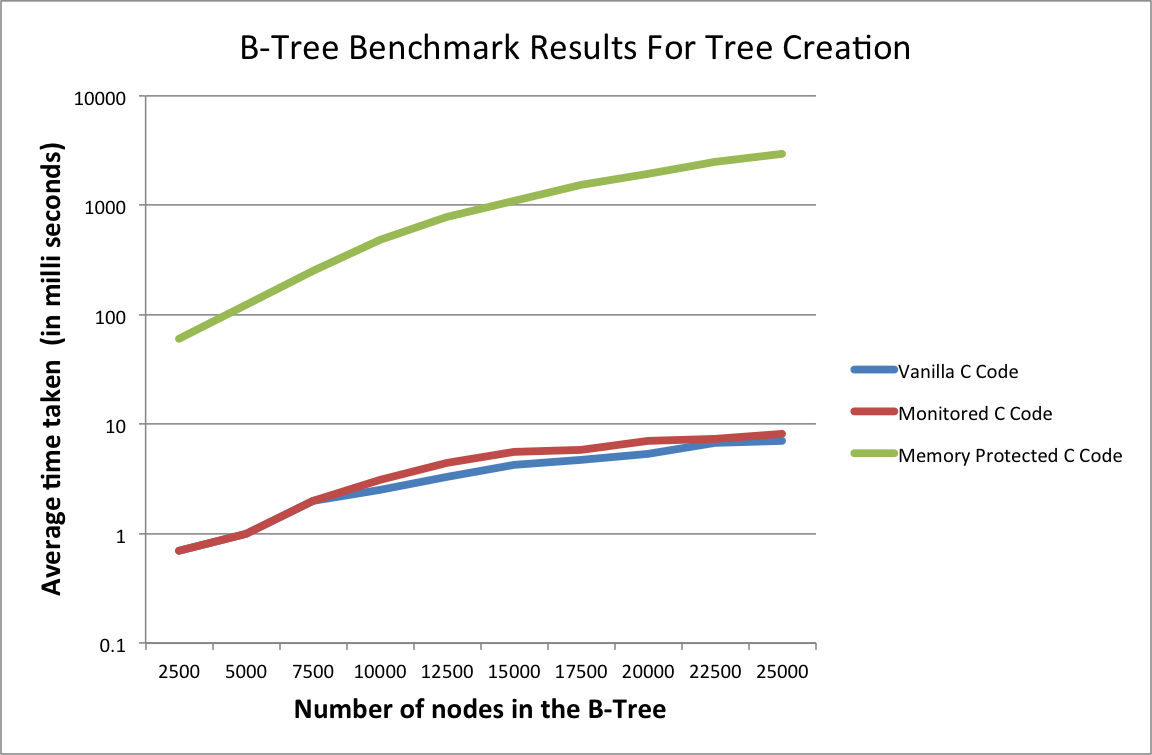
\includegraphics[scale=0.4]{./images/create.png}
\end{figure}
\begin{figure}[!h]
\caption{B-Tree Benchmark Results For Read Workloads}
\label{fig:read}
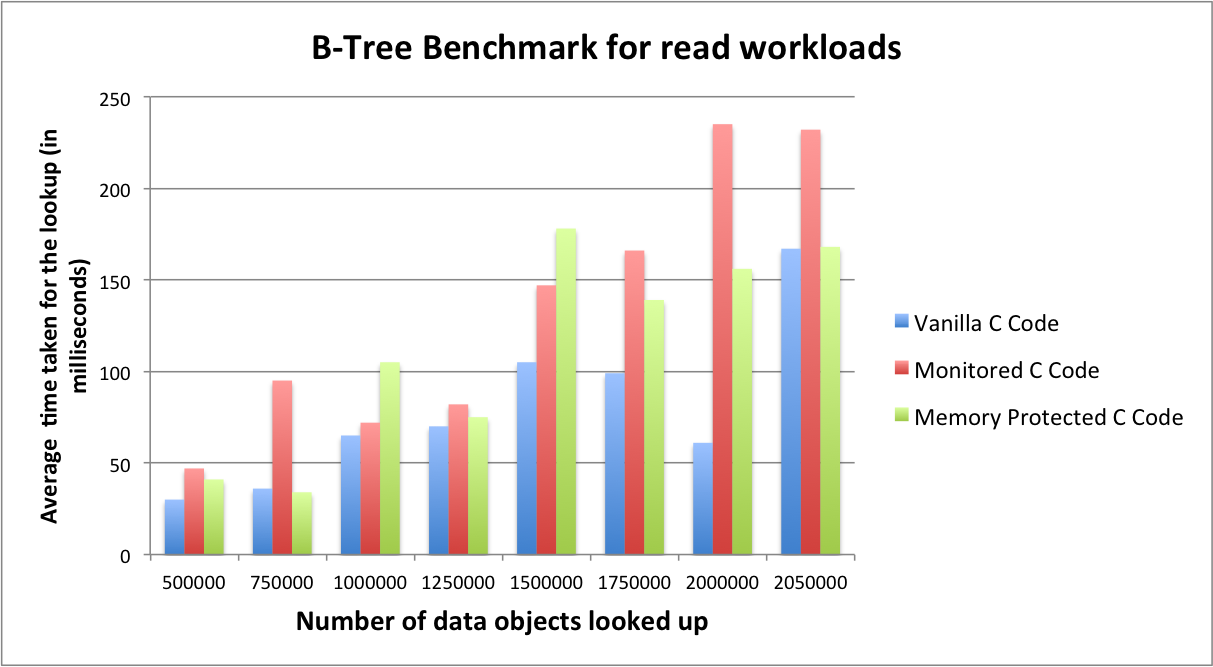
\includegraphics[scale=0.4]{./images/read.png}
\end{figure}
\begin{figure}[!h]
\caption{B-Tree Benchmark Results For Update Workloads}
\label{fig:update}
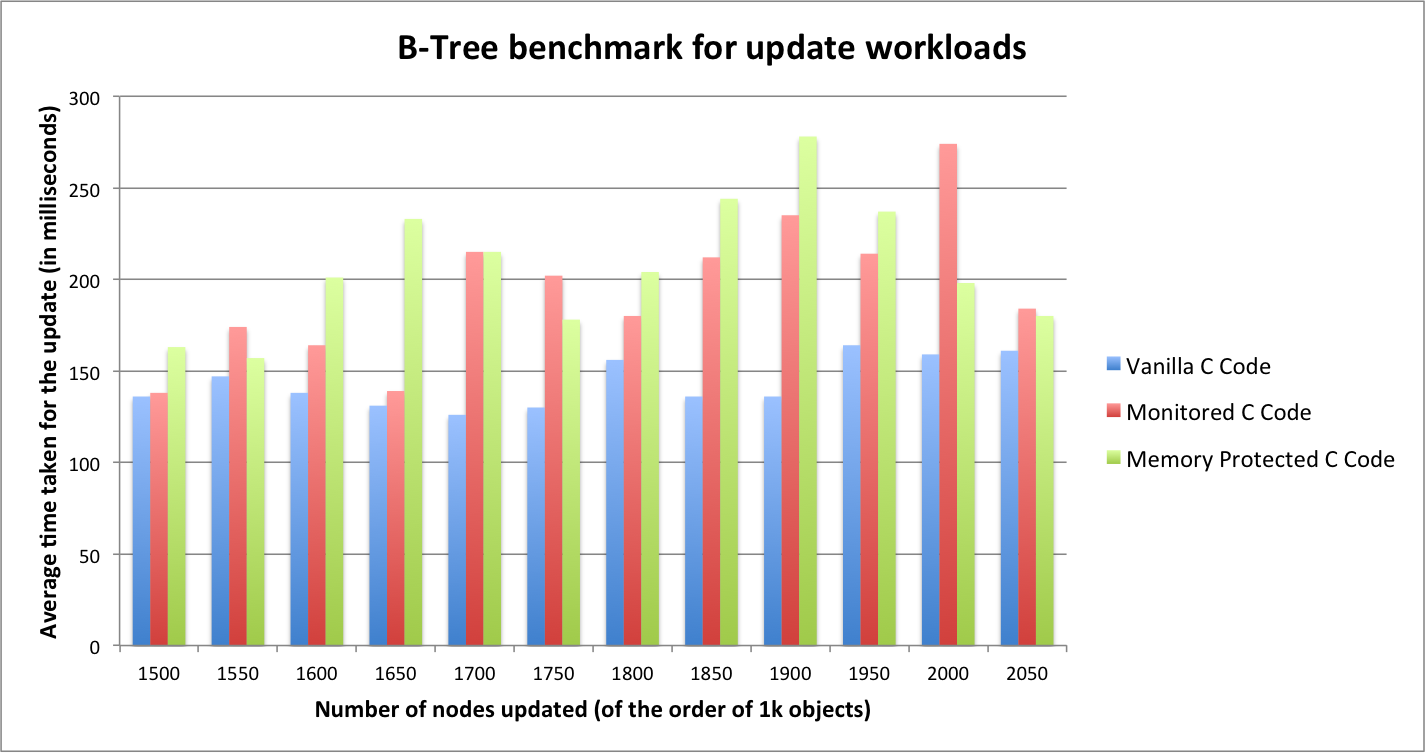
\includegraphics[scale=0.4]{./images/update.png}
\end{figure}
  

\paragraph{B-Tree Read Tests}
The second set of tests measures the overall overhead incurred in reading a set of random objects from a B-Tree of a fixed size (number of nodes in the binary tree was kept to 2500). For the read tests, we generate a random number of keys and search them in a preconstructed binary tree. We vary the number of keys read from 500, 000 to 2 million per experiment. Each data point is an average of 10 different experiments. Tracer has a reasonable overhead (of around $40\%$) over the vanilla C implementation. Page protection mechanism has an overhead of $28\%$ (refer to Fig. \ref{fig:read}}). 
Tracer performs a fine grained monitoring, whereas page protection mechanisms provide an approximation of the access pattern of the application. Subsequently, Tracer has slightly larger overheads over page protected mechanisms. However, these overheads are reasonable considering the information which our tracing tool provides the developer with.

\paragraph{B-Tree Update Tests}
The third set of tests measure the overall overhead incurred for update intensive workloads. As in the read test, we generate a random set of key pairs. Each key pair has a source and a destination key. The source key is searched in the binary tree and its value is updated with the destination keys value. If the source key is not found in the binary tree the update procedure returns. We vary the number of update operations from 1.5 million to 2.5 million for our tests. Tracer improves the performance of the update operations over page protected mechanism by $6.28\%$. The overhead over a vanilla C implementation is around $35\%$ %(refer to Fig. \ref{fig:b-tree\_update.png}).
 These tests indicate that Tracer performs well in comparison to page protection mechanism for update heavy workloads. 

\paragraph{B-Tree Traversal Tests}
The fourth set of experiments explore the performance of tree traversals for the three different mechanisms. Tree traversals are generally observed heavily for range queries in databases. Page protected mechanisms perform poorly for such workloads with over 2 orders of magnitude of overheads. 

\paragraph{}
The observation from the tree traversal and creation tests is that page protection mechanisms perform poorly when a large number of nodes of the tree are touched. This could be explained because such an access pattern would result in a high "{\emph{object flux}}" between the page buffer and page table. The movement of an object between the page table and page buffer involves page eviction and page materialization which have high overheads. Tracer circumvents these overheads by its interception and tagged counter based approach. 